\documentclass[11pt]{article}
\usepackage[hmargin=1in,vmargin=1in]{geometry}
\usepackage{xcolor}
\usepackage{algorithm2e}
\usepackage{tikz}
\usepackage{forest}

\usetikzlibrary{positioning}
\usepackage{amsmath,amssymb,amsfonts,url,sectsty,framed,tcolorbox,framed}
\newcommand{\pf}{{\bf Proof: }}
\newtheorem{theorem}{Theorem}
\newtheorem{lemma}{Lemma}
\newtheorem{proposition}{Proposition}
\newtheorem{definition}{Definition}
\newtheorem{remark}{Remark}
\newcommand{\qed}{\hfill \rule{2mm}{2mm}}

\begin{document}
%%%%%%%%%%%%%%%%%%%%%%%%%%%%%%%%%%%%%%%%%%%%%%%%%%%%%%%%%%%%%%%%%%%%%
\noindent
\rule{\textwidth}{1pt}
\begin{center}
{\bf [CS304] Introduction to Cryptography and Network Security}
\end{center}
Course Instructor: Dr. Dibyendu Roy \hfill Winter 2023-2024\\
Scribed by: Sanidhya Kumar (202151138) \hfill Lecture (Week 6)
\\
\rule{\textwidth}{1pt}
%%%%%%%%%%%%%%%%%%%%%%%%%%%%%%%%%%%%%%%%%%%%%%%%%%%%%%%%%%%
%write here

\section{Pseudo Random Bit Generator}
\[F(K, IV) = Z_i \text{ where } Z_i \in \{0, 1\}\]
Where \(K\) is the secret key and \(IV\) is the initialization vector.
Function \(F\) produces \(n\) bits \(Z_0, Z_1, ..., Z_{n-1}\).
\noindent\\\\
\textbf{Plaintext:} \(m_0, m_1, ..., m_{n-1}\) \\\\
\(\textbf{Z: } Z_0, Z_1, ..., Z_{n-1}\)\\\\
\textbf{Encryption:}
\[C_0 = m_0 \oplus Z_0,\]
\[C_1 = m_1 \oplus Z_1, \ldots,\]
\[C_{n-1} = m_{n-1} \oplus Z_{n-1}\]\\
\textbf{This function has the following properties:}
\begin{enumerate}
    \item The output \(Z_0, Z_1, ..., Z_{n-1}\) is a random-looking string. A "random-looking string" behaves like a sequence of random outcomes, such as coin tosses. Given such a string, it's impossible to discern whether it was produced by genuine randomness or by a pseudo-random generator with specific inputs. However, this string can be replicated precisely by applying the same inputs to a function, indicating its pseudo-random nature.
    \item If we provide the same input (\(K\), \(IV\)) to \(F\) at different times, it will produce the same \(Z_i\).

    \begin{center}
        \tikzset{every picture/.style={line width=0.75pt}} 
        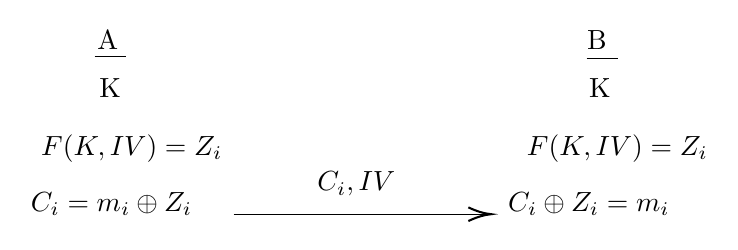
\begin{tikzpicture}[x=0.75pt,y=0.75pt,yscale=-1,xscale=1]
            \draw    (139,71.6) -- (154,71.6) ;
            \draw    (376,72.6) -- (391,72.6) ; 
            \draw    (206,147.6) -- (328,147.6) ;
            \draw [shift={(330,147.6)}, rotate = 180] [color={rgb, 255:red, 0; green, 0; blue, 0 }  ][line width=0.75]    (10.93,-3.29) .. controls (6.95,-1.4) and (3.31,-0.3) .. (0,0) .. controls (3.31,0.3) and (6.95,1.4) .. (10.93,3.29)   ;
            
            \draw (139,58) node [anchor=north west][inner sep=0.75pt]   [align=left] {A};
            \draw (375,58) node [anchor=north west][inner sep=0.75pt]   [align=left] {B};
            \draw (140,81) node [anchor=north west][inner sep=0.75pt]   [align=left] {K};
            \draw (376,81) node [anchor=north west][inner sep=0.75pt]   [align=left] {K};
            \draw (112,108) node [anchor=north west][inner sep=0.75pt]   [align=left] {$F(K,IV) = Z_i$};
            \draw (346,108) node [anchor=north west][inner sep=0.75pt]   [align=left] {$F(K,IV) = Z_i$};
            \draw (107,136) node [anchor=north west][inner sep=0.75pt]   [align=left] {$C_i = m_i \oplus Z_i$};
            \draw (337,136) node [anchor=north west][inner sep=0.75pt]   [align=left] {$C_i \oplus Z_i = m_i$};
            \draw (245,126) node [anchor=north west][inner sep=0.75pt]   [align=left] {$C_i, IV$};
        \end{tikzpicture}
    \end{center}    
    
    \item If a randomly selected secret key \(K\) is used, then the outputs \(Z_0, Z_1, ..., Z_{n-1}\) will be indistinguishable from a bit string generated by a random bit generator (coin tossing).
    \item \(F(K,IV)=Z_i\), \(0 \leq i \leq n\), the length of the output will be much greater than the length of \(K\). There exist efficient functions capable of producing an output of length \(2^{80} - 1\) for a key of length 80 bits. Leveraging this property, a relatively small key can encrypt exceedingly large messages.
    \item If we modify at least one bit of \(K\) or of \(IV\), then there will be an unpredictable change in the output of \(Z_i\).
    \[F(K, IV_1) = Z^{(1)}_i, \quad 0 \leq i \leq n - 1\]
    \[F(K, IV_2) = Z^{(2)}_i, \quad 0 \leq i \leq n - 1\]
    \(Z^{(1)}_i\) and \(Z^{(2)}_i\) are uncorrelated.

    \begin{center}
        \tikzset{every picture/.style={line width=0.75pt}} 
        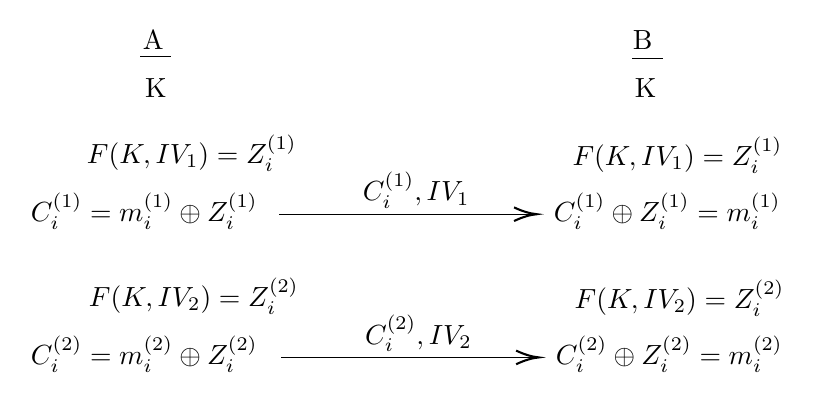
\begin{tikzpicture}[x=0.75pt,y=0.75pt,yscale=-1,xscale=1] 
            \draw    (139,71.6) -- (154,71.6) ;
            \draw    (376,72.6) -- (391,72.6) ;
            \draw    (206,147.6) -- (328,147.6) ;
            \draw [shift={(330,147.6)}, rotate = 180] [color={rgb, 255:red, 0; green, 0; blue, 0 }  ][line width=0.75]    (10.93,-3.29) .. controls (6.95,-1.4) and (3.31,-0.3) .. (0,0) .. controls (3.31,0.3) and (6.95,1.4) .. (10.93,3.29)   ;
            \draw    (207,216.6) -- (329,216.6) ;
            \draw [shift={(331,216.6)}, rotate = 180] [color={rgb, 255:red, 0; green, 0; blue, 0 }  ][line width=0.75]    (10.93,-3.29) .. controls (6.95,-1.4) and (3.31,-0.3) .. (0,0) .. controls (3.31,0.3) and (6.95,1.4) .. (10.93,3.29)   ;
            
            \draw (139,58) node [anchor=north west][inner sep=0.75pt]   [align=left] {A};
            \draw (375,58) node [anchor=north west][inner sep=0.75pt]   [align=left] {B};
            \draw (140,81) node [anchor=north west][inner sep=0.75pt]   [align=left] {K};
            \draw (376,81) node [anchor=north west][inner sep=0.75pt]   [align=left] {K};
            \draw (112,108) node [anchor=north west][inner sep=0.75pt]   [align=left] {$F(K,IV_1) = Z_i^{(1)}$};
            \draw (346,109) node [anchor=north west][inner sep=0.75pt]   [align=left] {$F(K,IV_1) = Z_i^{(1)}$};
            \draw (85,136) node [anchor=north west][inner sep=0.75pt]   [align=left] {$C_i^{(1)} = m_i^{(1)} \oplus Z_i^{(1)}$};
            \draw (337,136) node [anchor=north west][inner sep=0.75pt]   [align=left] {$C_i^{(1)} \oplus Z_i^{(1)} = m_i^{(1)}$};
            \draw (245,126) node [anchor=north west][inner sep=0.75pt]   [align=left] {$C_i^{(1)}, IV_1$};
            \draw (113,177) node [anchor=north west][inner sep=0.75pt]   [align=left] {$F(K,IV_2) = Z_i^{(2)}$};
            \draw (347,178) node [anchor=north west][inner sep=0.75pt]   [align=left] {$F(K,IV_2) = Z_i^{(2)}$};
            \draw (85,205) node [anchor=north west][inner sep=0.75pt]   [align=left] {$C_i^{(2)} = m_i^{(2)} \oplus Z_i^{(2)}$};
            \draw (338,205) node [anchor=north west][inner sep=0.75pt]   [align=left] {$C_i^{(2)} \oplus Z_i^{(2)} = m_i^{(2)}$};
            \draw (246,195) node [anchor=north west][inner sep=0.75pt]   [align=left] {$C_i^{(2)}, IV_2$};
        \end{tikzpicture}
    \end{center}    
    This property allows for the encryption of two distinct messages using the same key. By varying the initialization vector (IV), different \(Z_i\) values can be generated while utilizing the same key
    .
\end{enumerate}




\section{Stream Ciphers}

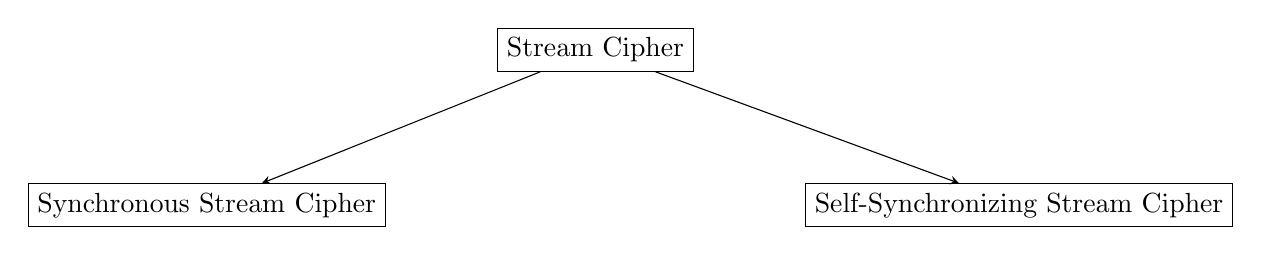
\begin{tikzpicture}[node distance=2cm]
    \node[draw, rectangle] (cipher) {Stream Cipher};
    \node[draw, rectangle, below left=of cipher] (sync) {Synchronous Stream Cipher};
    \node[draw, rectangle, below right=of cipher] (self) {Self-Synchronizing Stream Cipher};
    
    \draw[-stealth] (cipher) -- (sync);
    \draw[-stealth] (cipher) -- (self);
\end{tikzpicture}

\subsection{Synchronous Stream Cipher}
A synchronous stream cipher is one in which the key stream is generated independently of the plaintext bits and the ciphertext bits.\\\\
It has the following functions:
\begin{itemize}
    \item State Update function $\Rightarrow S_{i+1} = f(S_i , K)$ 
    \item Keystream Generator function $\Rightarrow Z_i = g(S_i , K)$ 
    \item Ciphertext Generation Function $\Rightarrow C_i = h(Z_i , m_i)$
\end{itemize}
\noindent
Here $S_0$ is the initial state and may be determined from $K$ and $IV$.

\subsection{Self-Synchronizing Stream Cipher}
A self-synchronizing stream cipher is one in which the keystream bits are generated as a function of the key and a fixed number of previous ciphertext bits.\\\\
It has the following functions:
\begin{itemize}
    \item $\sigma_i = (C_{i-t}, C_{i-t+1}, ..., C_{i-1})$
    \item State Update Function: $\sigma_{i+1} = f(\sigma, K, IV)$ where $\sigma = (C_{i-t}, C_{i-t+1}, ..., C_{i-1})$
    \item Keystream Generation Function: $Z_i = g(\sigma_i , K)$ 
    \item Ciphertext Generation Function: $C_i = h(Z_i , m_i)$
\end{itemize}
\noident
Here, $\sigma_0 = (C_{-t}, C_{-t+1}, ..., C_{-1})$ is the non-secret initial state.


\section{Linear Feedback Shift Register (LFSR)}

This setup comprises an $n$-bit register, with states represented by $S$ and individual bits by $s$. With each clock cycle, the register undergoes an update, generating an output (keystream bit) that can be used for encrypting messages.\\\\
A register of length $n$ implies it is an $n$-bit Linear Feedback Shift Register (LFSR), indicating it has a state of length $n$. At clock cycle $t = 0$, the register's state is labeled as $S_0$, where each bit $s_i$ for $0 \leq i \leq n - 1$ can take values from the set $\{0, 1\}$.
\begin{center}
    \tikzset{every picture/.style={line width=0.75pt}} 

    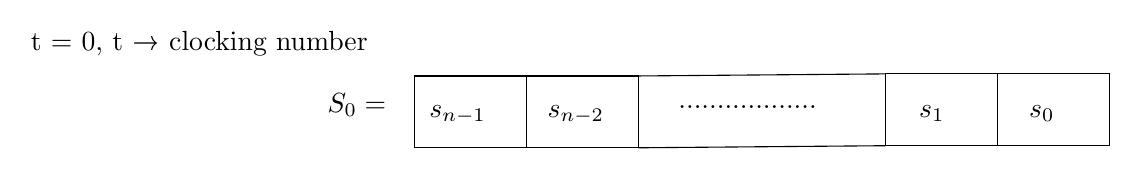
\begin{tikzpicture}[x=0.75pt,y=0.75pt,yscale=-1,xscale=1]
        \draw   (208,107) -- (262,107) -- (262,141.6) -- (208,141.6) -- cycle ; 
        \draw   (262,107) -- (316,107) -- (316,141.6) -- (262,141.6) -- cycle ;
        \draw   (435,106) -- (489,106) -- (489,140.6) -- (435,140.6) -- cycle ;
        \draw    (316,107) -- (435,106) ;
        \draw   (489,106) -- (543,106) -- (543,140.6) -- (489,140.6) -- cycle ;
        \draw    (316,141.6) -- (435,140.6) ;
        
        \draw (214,120) node [anchor=north west][inner sep=0.75pt]   [align=left] {$s_{n-1}$};
        \draw (271,120) node [anchor=north west][inner sep=0.75pt]   [align=left] {$s_{n-2}$};
        \draw (334,120) node [anchor=north west][inner sep=0.75pt]   [align=left] {..................};
        \draw (450,120) node [anchor=north west][inner sep=0.75pt]   [align=left] {$s_1$};
        \draw (503,120) node [anchor=north west][inner sep=0.75pt]   [align=left] {$s_0$};
        \draw (22,84) node [anchor=north west][inner sep=0.75pt]   [align=left] {t = 0, t → clocking number};
        \draw (165,114) node [anchor=north west][inner sep=0.75pt]   [align=left] {$S_0 = $};
    \end{tikzpicture}
\end{center}
\noindent
At each clocking number, a right shift by one bit takes place:
\begin{center}
    \tikzset{every picture/.style={line width=0.75pt}} 
    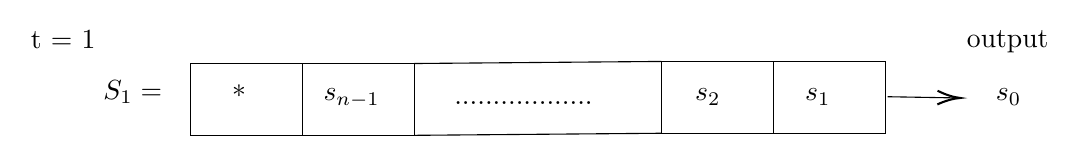
\begin{tikzpicture}[x=0.75pt,y=0.75pt,yscale=-1,xscale=1]
        \draw   (135,197) -- (189,197) -- (189,231.6) -- (135,231.6) -- cycle ;
        \draw   (189,197) -- (243,197) -- (243,231.6) -- (189,231.6) -- cycle ; 
        \draw   (362,196) -- (416,196) -- (416,230.6) -- (362,230.6) -- cycle ;
        \draw    (243,197) -- (362,196) ;
        \draw   (416,196) -- (470,196) -- (470,230.6) -- (416,230.6) -- cycle ;
        \draw    (243,231.6) -- (362,230.6) ;
        \draw    (471,213) -- (504,213.57) ;
        \draw [shift={(506,213.6)}, rotate = 180.98] [color={rgb, 255:red, 0; green, 0; blue, 0 }  ][line width=0.75]    (10.93,-3.29) .. controls (6.95,-1.4) and (3.31,-0.3) .. (0,0) .. controls (3.31,0.3) and (6.95,1.4) .. (10.93,3.29)   ;
        
        \draw (154,206) node [anchor=north west][inner sep=0.75pt]   [align=left] {*};
        \draw (198,208) node [anchor=north west][inner sep=0.75pt]   [align=left] {$s_{n-1}$};
        \draw (261,214) node [anchor=north west][inner sep=0.75pt]   [align=left] {..................};
        \draw (377,208) node [anchor=north west][inner sep=0.75pt]   [align=left] {$s_2$};
        \draw (430,208) node [anchor=north west][inner sep=0.75pt]   [align=left] {$s_1$};
        \draw (57,180) node [anchor=north west][inner sep=0.75pt]   [align=left] {t = 1};
        \draw (92,204) node [anchor=north west][inner sep=0.75pt]   [align=left] {$S_1 =$};
        \draw (508,180) node [anchor=north west][inner sep=0.75pt]   [align=left] {output};
        \draw (522,208) node [anchor=north west][inner sep=0.75pt]   [align=left] {$s_0$};
        
    \end{tikzpicture}
\end{center}
The rightmost bit $s_0$ serves as the output (the keystream bit), while the leftmost bit $s_n$ becomes empty. The leftmost bit, $s_n$, is referred to as the feedback bit, and its value is determined by a function $L$ applied to the entire state $S_0$, calculated as:
\[ s_n = L(s_0, s_1, \dots, s_{n-1}) = L(S_0) \]

\begin{center}
    \tikzset{every picture/.style={line width=0.75pt}} 
    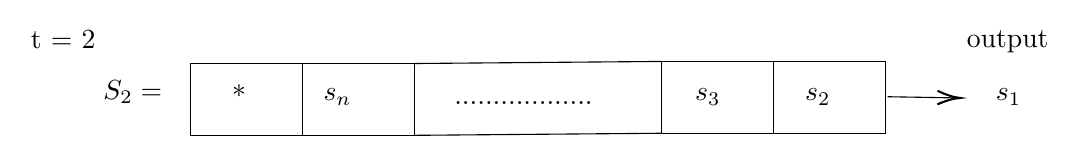
\begin{tikzpicture}[x=0.75pt,y=0.75pt,yscale=-1,xscale=1]
        \draw   (135,197) -- (189,197) -- (189,231.6) -- (135,231.6) -- cycle ;
        \draw   (189,197) -- (243,197) -- (243,231.6) -- (189,231.6) -- cycle ; 
        \draw   (362,196) -- (416,196) -- (416,230.6) -- (362,230.6) -- cycle ;
        \draw    (243,197) -- (362,196) ;
        \draw   (416,196) -- (470,196) -- (470,230.6) -- (416,230.6) -- cycle ;
        \draw    (243,231.6) -- (362,230.6) ;
        \draw    (471,213) -- (504,213.57) ;
        \draw [shift={(506,213.6)}, rotate = 180.98] [color={rgb, 255:red, 0; green, 0; blue, 0 }  ][line width=0.75]    (10.93,-3.29) .. controls (6.95,-1.4) and (3.31,-0.3) .. (0,0) .. controls (3.31,0.3) and (6.95,1.4) .. (10.93,3.29)   ;
        
        \draw (154,206) node [anchor=north west][inner sep=0.75pt]   [align=left] {*};
        \draw (198,208) node [anchor=north west][inner sep=0.75pt]   [align=left] {$s_n$};
        \draw (261,214) node [anchor=north west][inner sep=0.75pt]   [align=left] {..................};
        \draw (377,208) node [anchor=north west][inner sep=0.75pt]   [align=left] {$s_3$};
        \draw (430,208) node [anchor=north west][inner sep=0.75pt]   [align=left] {$s_2$};
        \draw (57,180) node [anchor=north west][inner sep=0.75pt]   [align=left] {t = 2};
        \draw (92,204) node [anchor=north west][inner sep=0.75pt]   [align=left] {$S_2 =$};
        \draw (508,180) node [anchor=north west][inner sep=0.75pt]   [align=left] {output};
        \draw (522,208) node [anchor=north west][inner sep=0.75pt]   [align=left] {$s_1$};
        
    \end{tikzpicture}
\end{center}

The feedback bit $s_{n+1} = L(S_1)$.

\begin{center}
    \tikzset{every picture/.style={line width=0.75pt}} 
    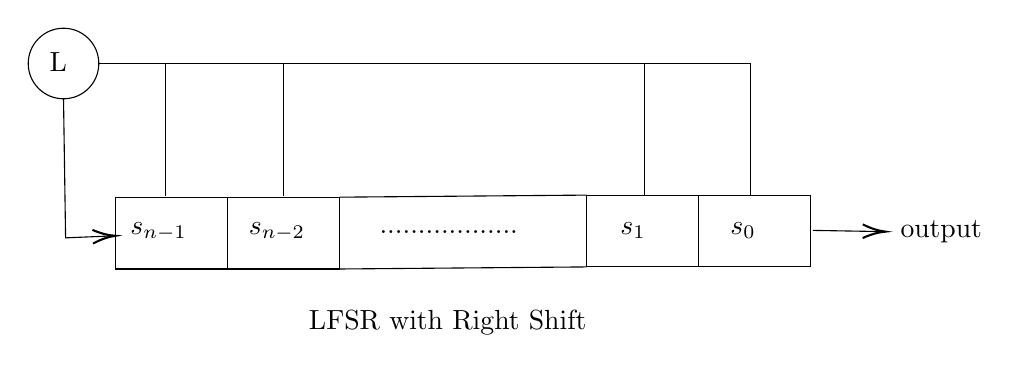
\begin{tikzpicture}[x=0.75pt,y=0.75pt,yscale=-1,xscale=1]
        \draw   (138,147) -- (192,147) -- (192,181.6) -- (138,181.6) -- cycle ;
        \draw   (192,147) -- (246,147) -- (246,181.6) -- (192,181.6) -- cycle ;
        \draw   (365,146) -- (419,146) -- (419,180.6) -- (365,180.6) -- cycle ; 
        \draw    (246,147) -- (365,146) ;
        \draw   (419,146) -- (473,146) -- (473,180.6) -- (419,180.6) -- cycle ;
        \draw    (246,181.6) -- (365,180.6) ; 
        \draw    (474,163) -- (507,163.57) ;
        \draw [shift={(509,163.6)}, rotate = 180.98] [color={rgb, 255:red, 0; green, 0; blue, 0 }  ][line width=0.75]    (10.93,-3.29) .. controls (6.95,-1.4) and (3.31,-0.3) .. (0,0) .. controls (3.31,0.3) and (6.95,1.4) .. (10.93,3.29)   ;
        \draw    (130,82.6) -- (444,82.6) -- (444,146) ;
        \draw   (96,82.6) .. controls (96,73.21) and (103.61,65.6) .. (113,65.6) .. controls (122.39,65.6) and (130,73.21) .. (130,82.6) .. controls (130,91.99) and (122.39,99.6) .. (113,99.6) .. controls (103.61,99.6) and (96,91.99) .. (96,82.6) -- cycle ;
        \draw    (113,99.6) -- (114,166.6) -- (136,165.68) ;
        \draw [shift={(138,165.6)}, rotate = 177.61] [color={rgb, 255:red, 0; green, 0; blue, 0 }  ][line width=0.75]    (10.93,-3.29) .. controls (6.95,-1.4) and (3.31,-0.3) .. (0,0) .. controls (3.31,0.3) and (6.95,1.4) .. (10.93,3.29)   ;
        \draw    (162,82.6) -- (162,146.6) ;
        \draw    (219,82.6) -- (219,146.6) ;
        \draw    (393,82.6) -- (393,146.6) ;
        
        \draw (144,158) node [anchor=north west][inner sep=0.75pt]   [align=left] {$s_{n-1}$};
        \draw (201,158) node [anchor=north west][inner sep=0.75pt]   [align=left] {$s_{n-2}$};
        \draw (264,162) node [anchor=north west][inner sep=0.75pt]   [align=left] {..................};
        \draw (380,158) node [anchor=north west][inner sep=0.75pt]   [align=left] {$s_1$};
        \draw (433,158) node [anchor=north west][inner sep=0.75pt]   [align=left] {$s_0$};
        \draw (515,157) node [anchor=north west][inner sep=0.75pt]   [align=left] {output};
        \draw (105,76) node [anchor=north west][inner sep=0.75pt]   [align=left] {L};
        \draw (230,200) node [anchor=north west][inner sep=0.75pt]   [align=left] {LFSR with Right Shift};
    \end{tikzpicture}
\end{center}
\noindent
The function $L$ is a linear function on the bits of the previous state. $L : \{0, 1\}^n \rightarrow \{0, 1\}$, $L(s_0, s_1, \dots, s_{n-1}) = s_n$.\\\\
A linear function can be represented as:
\[ L_a = a_0 \cdot s_0 \oplus a_1 \cdot s_1 \oplus \dots \oplus a_{n-1} \cdot s_{n-1} \text{ where } a_i \in \{0, 1\} \]\\
Suppose, an arbitrary function $L$ be defined as:
\[ L = a_0 \cdot s_0 \oplus a_1 \cdot s_1 \oplus \dots \oplus a_{n-1} \cdot s_{n-1} \oplus a_n \text{ where } a_i \in \{0, 1\} \]\\
In this function, if $a_n = 0$ then $L = L_a$, a linear function. Otherwise, if $a_n = 1$ then $L \neq L_a$. In fact, such a function is known as Affine function.\\

\fbox{\parbox{\linewidth}{
{\textbf{Function's Linearity\\}}

A function's linearity can be demonstrated by the property:
\[ L(X) \oplus L(Y) = L(X \oplus Y) \]
which implies that $L(X) \oplus L(Y) \oplus L(X \oplus Y)$ equals 0.
}}


\subsubsection*{Example 01:}

Check if the functions are linear or not. Solve it considering 2-bit inputs. 
\begin{enumerate}
    \item $L_1(x, y) = x \oplus y$
    \item $L_2(x, y) = 1 \oplus x \oplus y$
\end{enumerate}
\begin{align*}
    &\text{Compute } L_1(x) \oplus L_1(y) \oplus L_1(x \oplus y) \\
    &L_1(x) \oplus L_1(y) \oplus L_1(x \oplus y) = (x_1 \oplus x_2) \oplus (y_1 \oplus y_2) \oplus ((x_1 \oplus y_1) \oplus (x_2 \oplus y_2)) \\
    &L_1(x) \oplus L_1(y) \oplus L_1(x \oplus y) = 0 \\
    &\text{Therefore, } L_1 \text{ is a linear function.} \\
    \\
    &L_2(x) \oplus L_2(y) \oplus L_2(x \oplus y) = (1 \oplus x_1 \oplus x_2) \oplus (1 \oplus y_1 \oplus y_2) \oplus (1 \oplus (x_1 \oplus y_1) \oplus (x_2 \oplus y_2)) \\
    &L_2(x) \oplus L_2(y) \oplus L_2(x \oplus y) = 1 \\
    &\text{Therefore, } L_2 \text{ is not a linear function.}
\end{align*}

\subsection*{Example 02:}

Consider a 3 bit LFSR. $L= s_0 \oplus s_2$

\begin{center}
    \tikzset{every picture/.style={line width=0.75pt}}
    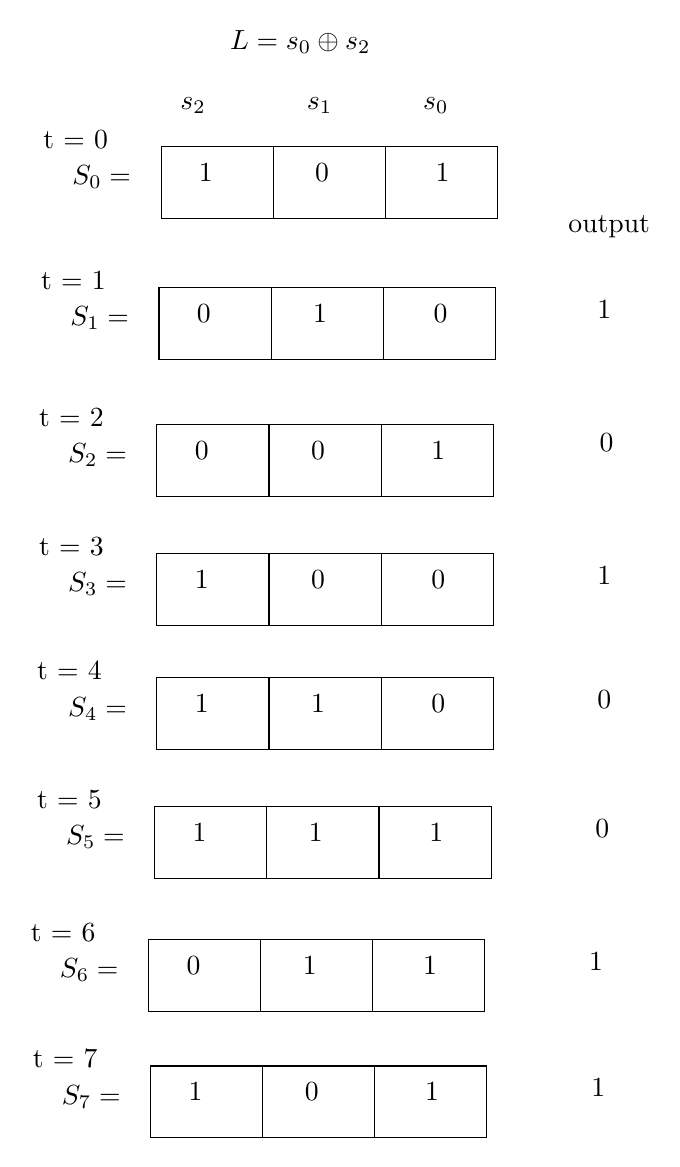
\begin{tikzpicture}[x=0.75pt,y=0.75pt,yscale=-1,xscale=1]
        
        \draw   (230,277) -- (284,277) -- (284,311.6) -- (230,311.6) -- cycle ;
        \draw   (284,277) -- (338,277) -- (338,311.6) -- (284,311.6) -- cycle ;
        \draw   (338,277) -- (392,277) -- (392,311.6) -- (338,311.6) -- cycle ;
        \draw   (229,345) -- (283,345) -- (283,379.6) -- (229,379.6) -- cycle ;
        \draw   (283,345) -- (337,345) -- (337,379.6) -- (283,379.6) -- cycle ;
        \draw   (337,345) -- (391,345) -- (391,379.6) -- (337,379.6) -- cycle ;
        \draw   (228,411) -- (282,411) -- (282,445.6) -- (228,445.6) -- cycle ;
        \draw   (282,411) -- (336,411) -- (336,445.6) -- (282,445.6) -- cycle ;
        \draw   (336,411) -- (390,411) -- (390,445.6) -- (336,445.6) -- cycle ;
        \draw   (228,473) -- (282,473) -- (282,507.6) -- (228,507.6) -- cycle ;
        \draw   (282,473) -- (336,473) -- (336,507.6) -- (282,507.6) -- cycle ;
        \draw   (336,473) -- (390,473) -- (390,507.6) -- (336,507.6) -- cycle ;
        \draw   (228,533) -- (282,533) -- (282,567.6) -- (228,567.6) -- cycle ;
        \draw   (282,533) -- (336,533) -- (336,567.6) -- (282,567.6) -- cycle ;
        \draw   (336,533) -- (390,533) -- (390,567.6) -- (336,567.6) -- cycle ;
        \draw   (227,595) -- (281,595) -- (281,629.6) -- (227,629.6) -- cycle ;
        \draw   (281,595) -- (335,595) -- (335,629.6) -- (281,629.6) -- cycle ;
        \draw   (335,595) -- (389,595) -- (389,629.6) -- (335,629.6) -- cycle ;
        \draw   (224,659) -- (278,659) -- (278,693.6) -- (224,693.6) -- cycle ;
        \draw   (278,659) -- (332,659) -- (332,693.6) -- (278,693.6) -- cycle ;
        \draw   (332,659) -- (386,659) -- (386,693.6) -- (332,693.6) -- cycle ;
        \draw   (225,720) -- (279,720) -- (279,754.6) -- (225,754.6) -- cycle ;
        \draw   (279,720) -- (333,720) -- (333,754.6) -- (279,754.6) -- cycle ;
        \draw   (333,720) -- (387,720) -- (387,754.6) -- (333,754.6) -- cycle ;
        
        \draw (303,284) node [anchor=north west][inner sep=0.75pt]   [align=left] {0};
        \draw (262,220) node [anchor=north west][inner sep=0.75pt]   [align=left] {$L = s_0 \oplus s_2$};
        \draw (238,252) node [anchor=north west][inner sep=0.75pt]   [align=left] {$s_2$};
        \draw (299,252) node [anchor=north west][inner sep=0.75pt]   [align=left] {$s_1$};
        \draw (355,252) node [anchor=north west][inner sep=0.75pt]   [align=left] {$s_0$};
        \draw (172,268) node [anchor=north west][inner sep=0.75pt]   [align=left] {t = 0};
        \draw (186,285) node [anchor=north west][inner sep=0.75pt]   [align=left] {$S_0 = $};
        \draw (425,309) node [anchor=north west][inner sep=0.75pt]   [align=left] {output};
        \draw (247,284) node [anchor=north west][inner sep=0.75pt]   [align=left] {1};
        \draw (361,284) node [anchor=north west][inner sep=0.75pt]   [align=left] {1};
        \draw (302,352) node [anchor=north west][inner sep=0.75pt]   [align=left] {1};
        \draw (171,336) node [anchor=north west][inner sep=0.75pt]   [align=left] {t = 1};
        \draw (185,353) node [anchor=north west][inner sep=0.75pt]   [align=left] {$S_1 = $};
        \draw (246,352) node [anchor=north west][inner sep=0.75pt]   [align=left] {0};
        \draw (360,352) node [anchor=north west][inner sep=0.75pt]   [align=left] {0};
        \draw (301,418) node [anchor=north west][inner sep=0.75pt]   [align=left] {0};
        \draw (170,402) node [anchor=north west][inner sep=0.75pt]   [align=left] {t = 2};
        \draw (184,419) node [anchor=north west][inner sep=0.75pt]   [align=left] {$S_2 = $};
        \draw (245,418) node [anchor=north west][inner sep=0.75pt]   [align=left] {0};
        \draw (359,418) node [anchor=north west][inner sep=0.75pt]   [align=left] {1};
        \draw (301,480) node [anchor=north west][inner sep=0.75pt]   [align=left] {0};
        \draw (170,464) node [anchor=north west][inner sep=0.75pt]   [align=left] {t = 3};
        \draw (184,481) node [anchor=north west][inner sep=0.75pt]   [align=left] {$S_3 = $};
        \draw (245,480) node [anchor=north west][inner sep=0.75pt]   [align=left] {1};
        \draw (359,480) node [anchor=north west][inner sep=0.75pt]   [align=left] {0};
        \draw (439,350) node [anchor=north west][inner sep=0.75pt]   [align=left] {1};
        \draw (440,414) node [anchor=north west][inner sep=0.75pt]   [align=left] {0};
        \draw (439,478) node [anchor=north west][inner sep=0.75pt]   [align=left] {1};
        \draw (301,540) node [anchor=north west][inner sep=0.75pt]   [align=left] {1};
        \draw (169,524) node [anchor=north west][inner sep=0.75pt]   [align=left] {t = 4};
        \draw (184,541) node [anchor=north west][inner sep=0.75pt]   [align=left] {$S_4 = $};
        \draw (245,540) node [anchor=north west][inner sep=0.75pt]   [align=left] {1};
        \draw (359,540) node [anchor=north west][inner sep=0.75pt]   [align=left] {0};
        \draw (439,538) node [anchor=north west][inner sep=0.75pt]   [align=left] {0};
        \draw (300,602) node [anchor=north west][inner sep=0.75pt]   [align=left] {1};
        \draw (169,586) node [anchor=north west][inner sep=0.75pt]   [align=left] {t = 5};
        \draw (183,603) node [anchor=north west][inner sep=0.75pt]   [align=left] {$S_5 = $};
        \draw (244,602) node [anchor=north west][inner sep=0.75pt]   [align=left] {1};
        \draw (358,602) node [anchor=north west][inner sep=0.75pt]   [align=left] {1};
        \draw (438,600) node [anchor=north west][inner sep=0.75pt]   [align=left] {0};
        \draw (297,666) node [anchor=north west][inner sep=0.75pt]   [align=left] {1};
        \draw (166,650) node [anchor=north west][inner sep=0.75pt]   [align=left] {t = 6};
        \draw (180,667) node [anchor=north west][inner sep=0.75pt]   [align=left] {$S_6 = $};
        \draw (241,666) node [anchor=north west][inner sep=0.75pt]   [align=left] {0};
        \draw (355,666) node [anchor=north west][inner sep=0.75pt]   [align=left] {1};
        \draw (435,664) node [anchor=north west][inner sep=0.75pt]   [align=left] {1};
        \draw (298,727) node [anchor=north west][inner sep=0.75pt]   [align=left] {0};
        \draw (167,711) node [anchor=north west][inner sep=0.75pt]   [align=left] {t = 7};
        \draw (181,728) node [anchor=north west][inner sep=0.75pt]   [align=left] {$S_7 = $};
        \draw (242,727) node [anchor=north west][inner sep=0.75pt]   [align=left] {1};
        \draw (356,727) node [anchor=north west][inner sep=0.75pt]   [align=left] {1};
        \draw (436,725) node [anchor=north west][inner sep=0.75pt]   [align=left] {1};        
    \end{tikzpicture}
\end{center}

\noindent
In the given example, we observe that from the initial state at time $t=0$ to the state at $t=7$, all non-zero states are generated sequentially. Subsequently, after $t=7$, the output bits begin to repeat as the initial state is reached again. Therefore, the maximum achievable output length in this Linear Feedback Shift Register (LFSR) without repetition is 7. As a result, when employing an LFSR, the maximum number of non-zero states that can be generated is $2^{n-1}$, where $n$ represents the number of bits in the register.\\\\
Additionally, if the initial state is the all-zero state, signifying that all bits in the register are 0, it will persist in this zero state indefinitely. Consequently, in any LFSR, if the input state is 0, it will remain as zero.
\\
\subsection*{Example 03:}

Consider a 3 bit LFSR with $L=s_0$

\begin{center}   
    \tikzset{every picture/.style={line width=0.75pt}}
    \begin{tikzpicture}[x=0.75pt,y=0.75pt,yscale=-1,xscale=1]
        \draw   (230,277) -- (284,277) -- (284,311.6) -- (230,311.6) -- cycle ;
        \draw   (284,277) -- (338,277) -- (338,311.6) -- (284,311.6) -- cycle ; 
        \draw   (338,277) -- (392,277) -- (392,311.6) -- (338,311.6) -- cycle ; 
        \draw   (229,345) -- (283,345) -- (283,379.6) -- (229,379.6) -- cycle ;
        \draw   (283,345) -- (337,345) -- (337,379.6) -- (283,379.6) -- cycle ;
        \draw   (337,345) -- (391,345) -- (391,379.6) -- (337,379.6) -- cycle ;
        \draw   (228,411) -- (282,411) -- (282,445.6) -- (228,445.6) -- cycle ;
        \draw   (282,411) -- (336,411) -- (336,445.6) -- (282,445.6) -- cycle ;
        \draw   (336,411) -- (390,411) -- (390,445.6) -- (336,445.6) -- cycle ;
        \draw   (228,473) -- (282,473) -- (282,507.6) -- (228,507.6) -- cycle ;
        \draw   (282,473) -- (336,473) -- (336,507.6) -- (282,507.6) -- cycle ;
        \draw   (336,473) -- (390,473) -- (390,507.6) -- (336,507.6) -- cycle ;
        
        
        \draw (303,284) node [anchor=north west][inner sep=0.75pt]   [align=left] {0};
        \draw (290,220) node [anchor=north west][inner sep=0.75pt]   [align=left] {$L = s0$};
        \draw (238,252) node [anchor=north west][inner sep=0.75pt]   [align=left] {$s_2$};
        \draw (299,252) node [anchor=north west][inner sep=0.75pt]   [align=left] {$s_1$};
        \draw (355,252) node [anchor=north west][inner sep=0.75pt]   [align=left] {$s_0$};
        \draw (172,268) node [anchor=north west][inner sep=0.75pt]   [align=left] {t = 0};
        \draw (186,285) node [anchor=north west][inner sep=0.75pt]   [align=left] {$S_0 = $};
        \draw (425,309) node [anchor=north west][inner sep=0.75pt]   [align=left] {output};
        \draw (247,284) node [anchor=north west][inner sep=0.75pt]   [align=left] {1};
        \draw (361,284) node [anchor=north west][inner sep=0.75pt]   [align=left] {1};
        \draw (302,352) node [anchor=north west][inner sep=0.75pt]   [align=left] {1};
        \draw (171,336) node [anchor=north west][inner sep=0.75pt]   [align=left] {t = 1};
        \draw (185,353) node [anchor=north west][inner sep=0.75pt]   [align=left] {$S_1 = $};
        \draw (246,352) node [anchor=north west][inner sep=0.75pt]   [align=left] {1};
        \draw (360,352) node [anchor=north west][inner sep=0.75pt]   [align=left] {0};
        \draw (301,418) node [anchor=north west][inner sep=0.75pt]   [align=left] {1};
        \draw (170,402) node [anchor=north west][inner sep=0.75pt]   [align=left] {t = 2};
        \draw (184,419) node [anchor=north west][inner sep=0.75pt]   [align=left] {$S_2 = $};
        \draw (245,418) node [anchor=north west][inner sep=0.75pt]   [align=left] {0};
        \draw (359,418) node [anchor=north west][inner sep=0.75pt]   [align=left] {1};
        \draw (301,480) node [anchor=north west][inner sep=0.75pt]   [align=left] {0};
        \draw (170,464) node [anchor=north west][inner sep=0.75pt]   [align=left] {t = 3};
        \draw (184,481) node [anchor=north west][inner sep=0.75pt]   [align=left] {$S_3 = $};
        \draw (245,480) node [anchor=north west][inner sep=0.75pt]   [align=left] {1};
        \draw (359,480) node [anchor=north west][inner sep=0.75pt]   [align=left] {1};
        \draw (439,350) node [anchor=north west][inner sep=0.75pt]   [align=left] {1};
        \draw (440,414) node [anchor=north west][inner sep=0.75pt]   [align=left] {0};
        \draw (439,478) node [anchor=north west][inner sep=0.75pt]   [align=left] {1};        
    \end{tikzpicture}
\end{center}
\noindent
In this example, we can see that the initial state is reached again at $t=3$.

\subsection{Period of an LFSR}

If $S_0$ represents a non-zero state and $S_0$ recurs after $m$ clock cycles of the LFSR, then $m$ defines the period of the LFSR. An LFSR comprising $n$ bits can achieve a maximum period of $2^n - 1$.\\\\
Consider an LFSR where different non-zero states recur after varying numbers of clock cycles, labeled as $x_1$ states repeating after $P_1$ clock cycles, $x_2$ states repeating after $P_2$ clock cycles, and so on until $x_n$ states repeating after $P_n$ clock cycles. Here, each non-zero state is uniquely represented by one of the $x_i$'s. Consequently, any non-zero state will reappear after a certain number of clock cycles, belonging to the set $\{P_1, P_2, \dots, P_n\}$.\\\\
Hence, the period of the LFSR, defining the time it takes for the sequence to repeat, can be calculated by determining the least common multiple (LCM) of $P_1, P_2, \dots, P_n$. Thus, the period of the LFSR can be expressed as:
\textbf{\[\text{Period of LFSR} = \text{LCM}(P_1, P_2, \dots, P_n)\]}
\noindent
Consider a $n$-bit LFSR:
\begin{center}
    \tikzset{every picture/.style={line width=0.75pt}} 
    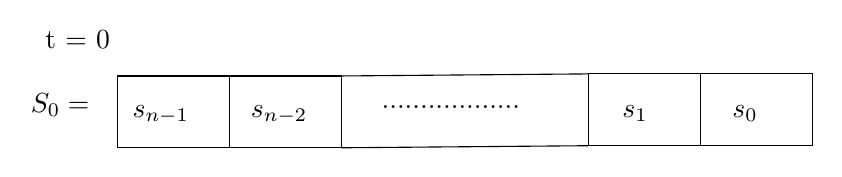
\begin{tikzpicture}[x=0.75pt,y=0.75pt,yscale=-1,xscale=1]
        \draw   (208,107) -- (262,107) -- (262,141.6) -- (208,141.6) -- cycle ; 
        \draw   (262,107) -- (316,107) -- (316,141.6) -- (262,141.6) -- cycle ;
        \draw   (435,106) -- (489,106) -- (489,140.6) -- (435,140.6) -- cycle ;
        \draw    (316,107) -- (435,106) ;
        \draw   (489,106) -- (543,106) -- (543,140.6) -- (489,140.6) -- cycle ;
        \draw    (316,141.6) -- (435,140.6) ;
        
        \draw (214,120) node [anchor=north west][inner sep=0.75pt]   [align=left] {$s_{n-1}$};
        \draw (271,120) node [anchor=north west][inner sep=0.75pt]   [align=left] {$s_{n-2}$};
        \draw (334,120) node [anchor=north west][inner sep=0.75pt]   [align=left] {..................};
        \draw (450,120) node [anchor=north west][inner sep=0.75pt]   [align=left] {$s_1$};
        \draw (503,120) node [anchor=north west][inner sep=0.75pt]   [align=left] {$s_0$};
        \draw (172,84) node [anchor=north west][inner sep=0.75pt]   [align=left] {t = 0};
        \draw (165,114) node [anchor=north west][inner sep=0.75pt]   [align=left] {$S_0 = $};
    \end{tikzpicture}
\end{center}
\noindent
After 1 clocking, $s_n$ will be:
\[ s_n = L(s_0, s_1, \dots, s_{n-1}) \]
\[ s_n = c_1 \cdot s_{n-1} \oplus c_2 \cdot s_{n-2} \oplus \dots \oplus c_n \cdot s_0 \quad \text{where } c_i \in \{0, 1\} \]
\noindent
To implement LFSR in hardware, we only need AND and XOR gates as shown below. The value of $s_i$ will be XORed or not depends on the value of $c_{n-i}$.

\begin{center}
    \tikzset{every picture/.style={line width=0.75pt}} 
    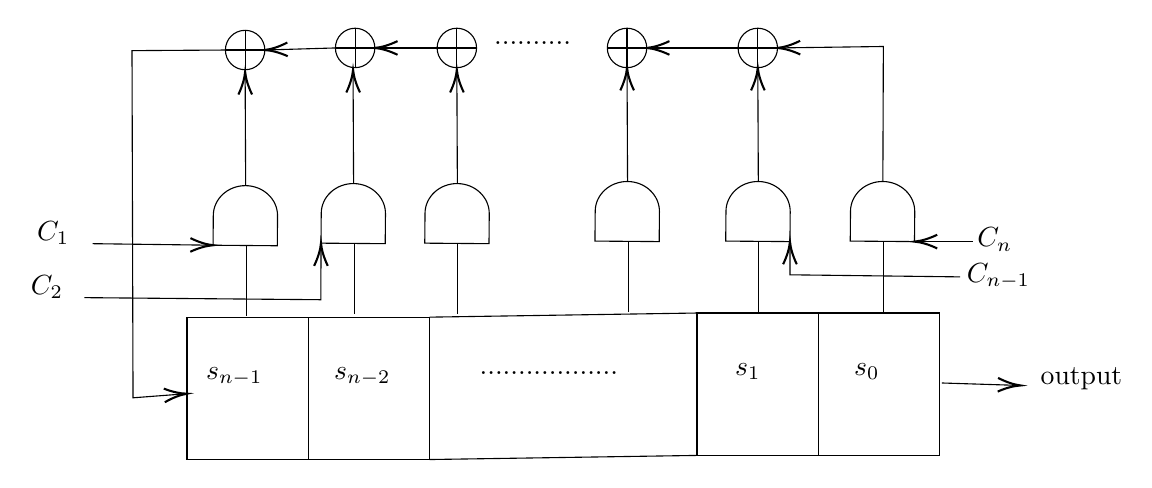
\begin{tikzpicture}[x=0.75pt,y=0.75pt,yscale=-1,xscale=1]
        \draw   (110.47,177.2) -- (168.93,177.2) -- (168.93,245.8) -- (110.47,245.8) -- cycle ;
        \draw   (168.93,177.2) -- (227.39,177.2) -- (227.39,245.8) -- (168.93,245.8) -- cycle ;
        \draw   (356.22,175.21) -- (414.68,175.21) -- (414.68,243.82) -- (356.22,243.82) -- cycle ; 
        \draw    (227.39,177.2) -- (356.22,175.21) ;
        \draw   (414.68,175.21) -- (473.14,175.21) -- (473.14,243.82) -- (414.68,243.82) -- cycle ;
        \draw    (227.39,245.8) -- (356.22,243.82) ;
        \draw    (474.22,208.92) -- (510.11,210.05) ;
        \draw [shift={(512.11,210.11)}, rotate = 181.8] [color={rgb, 255:red, 0; green, 0; blue, 0 }  ][line width=0.75]    (10.93,-3.29) .. controls (6.95,-1.4) and (3.31,-0.3) .. (0,0) .. controls (3.31,0.3) and (6.95,1.4) .. (10.93,3.29)   ;
        \draw    (129,48.5) -- (84,48.8) -- (84.49,216.06) -- (108.47,214.23) ;
        \draw [shift={(110.47,214.08)}, rotate = 175.64] [color={rgb, 255:red, 0; green, 0; blue, 0 }  ][line width=0.75]    (10.93,-3.29) .. controls (6.95,-1.4) and (3.31,-0.3) .. (0,0) .. controls (3.31,0.3) and (6.95,1.4) .. (10.93,3.29)   ;
        \draw   (370.05,140.55) -- (370.17,126.13) .. controls (370.24,118.17) and (377.22,111.77) .. (385.76,111.84) .. controls (394.31,111.91) and (401.18,118.42) .. (401.12,126.38) -- (401,140.8) -- cycle ;
        \draw    (386,140.8) -- (386,174.8) ; 
        \draw   (129,48.5) .. controls (129,43.25) and (133.25,39) .. (138.5,39) .. controls (143.75,39) and (148,43.25) .. (148,48.5) .. controls (148,53.75) and (143.75,58) .. (138.5,58) .. controls (133.25,58) and (129,53.75) .. (129,48.5) -- cycle ; \draw   (129,48.5) -- (148,48.5) ; \draw   (138.5,39) -- (138.5,58) ;
        \draw   (182,47.5) .. controls (182,42.25) and (186.25,38) .. (191.5,38) .. controls (196.75,38) and (201,42.25) .. (201,47.5) .. controls (201,52.75) and (196.75,57) .. (191.5,57) .. controls (186.25,57) and (182,52.75) .. (182,47.5) -- cycle ; \draw   (182,47.5) -- (201,47.5) ; \draw   (191.5,38) -- (191.5,57) ;
        \draw   (231,47.5) .. controls (231,42.25) and (235.25,38) .. (240.5,38) .. controls (245.75,38) and (250,42.25) .. (250,47.5) .. controls (250,52.75) and (245.75,57) .. (240.5,57) .. controls (235.25,57) and (231,52.75) .. (231,47.5) -- cycle ; \draw   (231,47.5) -- (250,47.5) ; \draw   (240.5,38) -- (240.5,57) ;
        \draw   (313,47.5) .. controls (313,42.25) and (317.25,38) .. (322.5,38) .. controls (327.75,38) and (332,42.25) .. (332,47.5) .. controls (332,52.75) and (327.75,57) .. (322.5,57) .. controls (317.25,57) and (313,52.75) .. (313,47.5) -- cycle ; \draw   (313,47.5) -- (332,47.5) ; \draw   (322.5,38) -- (322.5,57) ;
        \draw   (376,47.5) .. controls (376,42.25) and (380.25,38) .. (385.5,38) .. controls (390.75,38) and (395,42.25) .. (395,47.5) .. controls (395,52.75) and (390.75,57) .. (385.5,57) .. controls (380.25,57) and (376,52.75) .. (376,47.5) -- cycle ; \draw   (376,47.5) -- (395,47.5) ; \draw   (385.5,38) -- (385.5,57) ;
        \draw    (376,47.5) -- (334,47.5) ;
        \draw [shift={(332,47.5)}, rotate = 360] [color={rgb, 255:red, 0; green, 0; blue, 0 }  ][line width=0.75]    (10.93,-3.29) .. controls (6.95,-1.4) and (3.31,-0.3) .. (0,0) .. controls (3.31,0.3) and (6.95,1.4) .. (10.93,3.29)   ;
        \draw    (231,47.5) -- (203,47.5) ;
        \draw [shift={(201,47.5)}, rotate = 360] [color={rgb, 255:red, 0; green, 0; blue, 0 }  ][line width=0.75]    (10.93,-3.29) .. controls (6.95,-1.4) and (3.31,-0.3) .. (0,0) .. controls (3.31,0.3) and (6.95,1.4) .. (10.93,3.29)   ;
        \draw    (182,47.5) -- (150,48.44) ;
        \draw [shift={(148,48.5)}, rotate = 358.32] [color={rgb, 255:red, 0; green, 0; blue, 0 }  ][line width=0.75]    (10.93,-3.29) .. controls (6.95,-1.4) and (3.31,-0.3) .. (0,0) .. controls (3.31,0.3) and (6.95,1.4) .. (10.93,3.29)   ;
        \draw    (385.76,111.84) -- (385.51,59) ;
        \draw [shift={(385.5,57)}, rotate = 89.73] [color={rgb, 255:red, 0; green, 0; blue, 0 }  ][line width=0.75]    (10.93,-3.29) .. controls (6.95,-1.4) and (3.31,-0.3) .. (0,0) .. controls (3.31,0.3) and (6.95,1.4) .. (10.93,3.29)   ;
        \draw   (307.05,140.55) -- (307.17,126.13) .. controls (307.24,118.17) and (314.22,111.77) .. (322.76,111.84) .. controls (331.31,111.91) and (338.18,118.42) .. (338.12,126.38) -- (338,140.8) -- cycle ;
        \draw    (323,140.8) -- (323,174.8) ;
        \draw    (322.76,111.84) -- (322.51,59) ;
        \draw [shift={(322.5,57)}, rotate = 89.73] [color={rgb, 255:red, 0; green, 0; blue, 0 }  ][line width=0.75]    (10.93,-3.29) .. controls (6.95,-1.4) and (3.31,-0.3) .. (0,0) .. controls (3.31,0.3) and (6.95,1.4) .. (10.93,3.29)   ;
        \draw   (225.05,141.55) -- (225.17,127.13) .. controls (225.24,119.17) and (232.22,112.77) .. (240.76,112.84) .. controls (249.31,112.91) and (256.18,119.42) .. (256.12,127.38) -- (256,141.8) -- cycle ;
        \draw    (241,141.8) -- (241,175.8) ; 
        \draw    (240.76,112.84) -- (240.51,60) ;
        \draw [shift={(240.5,58)}, rotate = 89.73] [color={rgb, 255:red, 0; green, 0; blue, 0 }  ][line width=0.75]    (10.93,-3.29) .. controls (6.95,-1.4) and (3.31,-0.3) .. (0,0) .. controls (3.31,0.3) and (6.95,1.4) .. (10.93,3.29)   ;
        \draw   (175.05,141.55) -- (175.17,127.13) .. controls (175.24,119.17) and (182.22,112.77) .. (190.76,112.84) .. controls (199.31,112.91) and (206.18,119.42) .. (206.12,127.38) -- (206,141.8) -- cycle ;
        \draw    (191,141.8) -- (191,175.8) ; 
        \draw    (190.76,112.84) -- (190.51,60) ;
        \draw [shift={(190.5,58)}, rotate = 89.73] [color={rgb, 255:red, 0; green, 0; blue, 0 }  ][line width=0.75]    (10.93,-3.29) .. controls (6.95,-1.4) and (3.31,-0.3) .. (0,0) .. controls (3.31,0.3) and (6.95,1.4) .. (10.93,3.29)   ; 
        \draw   (123.05,142.55) -- (123.17,128.13) .. controls (123.24,120.17) and (130.22,113.77) .. (138.76,113.84) .. controls (147.31,113.91) and (154.18,120.42) .. (154.12,128.38) -- (154,142.8) -- cycle ;
        \draw    (139,142.8) -- (139,176.8) ;
        \draw    (138.76,113.84) -- (138.51,61) ;
        \draw [shift={(138.5,59)}, rotate = 89.73] [color={rgb, 255:red, 0; green, 0; blue, 0 }  ][line width=0.75]    (10.93,-3.29) .. controls (6.95,-1.4) and (3.31,-0.3) .. (0,0) .. controls (3.31,0.3) and (6.95,1.4) .. (10.93,3.29)   ;
        \draw   (430.05,140.55) -- (430.17,126.13) .. controls (430.24,118.17) and (437.22,111.77) .. (445.76,111.84) .. controls (454.31,111.91) and (461.18,118.42) .. (461.12,126.38) -- (461,140.8) -- cycle ;
        \draw    (446,140.8) -- (446,174.8) ;
        \draw    (445.76,111.84) -- (446,46.8) -- (397,47.47) ;
        \draw [shift={(395,47.5)}, rotate = 359.21] [color={rgb, 255:red, 0; green, 0; blue, 0 }  ][line width=0.75]    (10.93,-3.29) .. controls (6.95,-1.4) and (3.31,-0.3) .. (0,0) .. controls (3.31,0.3) and (6.95,1.4) .. (10.93,3.29)   ;
        \draw    (489,140.8) -- (463,140.8) ;
        \draw [shift={(461,140.8)}, rotate = 360] [color={rgb, 255:red, 0; green, 0; blue, 0 }  ][line width=0.75]    (10.93,-3.29) .. controls (6.95,-1.4) and (3.31,-0.3) .. (0,0) .. controls (3.31,0.3) and (6.95,1.4) .. (10.93,3.29)   ;
        \draw    (483,157.8) -- (401,156.8) -- (401,142.8) ;
        \draw [shift={(401,140.8)}, rotate = 90] [color={rgb, 255:red, 0; green, 0; blue, 0 }  ][line width=0.75]    (10.93,-3.29) .. controls (6.95,-1.4) and (3.31,-0.3) .. (0,0) .. controls (3.31,0.3) and (6.95,1.4) .. (10.93,3.29)   ;
        \draw    (61,167.8) -- (175,168.8) -- (175.05,143.55) ;
        \draw [shift={(175.05,141.55)}, rotate = 90.11] [color={rgb, 255:red, 0; green, 0; blue, 0 }  ][line width=0.75]    (10.93,-3.29) .. controls (6.95,-1.4) and (3.31,-0.3) .. (0,0) .. controls (3.31,0.3) and (6.95,1.4) .. (10.93,3.29)   ;
        \draw    (65,141.8) -- (121.05,142.52) ;
        \draw [shift={(123.05,142.55)}, rotate = 180.74] [color={rgb, 255:red, 0; green, 0; blue, 0 }  ][line width=0.75]    (10.93,-3.29) .. controls (6.95,-1.4) and (3.31,-0.3) .. (0,0) .. controls (3.31,0.3) and (6.95,1.4) .. (10.93,3.29)   ;
        
        \draw (118.41,200.39) node [anchor=north west][inner sep=0.75pt]   [align=left] {$s_{n-1}$};
        \draw (180.12,200.39) node [anchor=north west][inner sep=0.75pt]   [align=left] {$s_{n-2}$};
        \draw (250.22,202.38) node [anchor=north west][inner sep=0.75pt]   [align=left] {..................};
        \draw (373.32,198.41) node [anchor=north west][inner sep=0.75pt]   [align=left] {$s_1$};
        \draw (430.7,198.41) node [anchor=north west][inner sep=0.75pt]   [align=left] {$s_0$};
        \draw (520.55,200.39) node [anchor=north west][inner sep=0.75pt]   [align=left] {output};
        \draw (257.22,43.38) node [anchor=north west][inner sep=0.75pt]   [align=left] {..........};
        \draw (490,133) node [anchor=north west][inner sep=0.75pt]   [align=left] {$C_n$};
        \draw (485,150) node [anchor=north west][inner sep=0.75pt]   [align=left] {$C_{n-1}$};
        \draw (34,156) node [anchor=north west][inner sep=0.75pt]   [align=left] {$C_2$};
        \draw (37,130) node [anchor=north west][inner sep=0.75pt]   [align=left] {$C_1$};        
    \end{tikzpicture}
\end{center}
\noindent
\\Corresponding to every LFSR, we have a Linear Feedback Function (LFF). Corresponding to LFF, we can construct a polynomial $f(x)$.
\[ L = c_1 \cdot s_{n-1} \oplus c_2 \cdot s_{n-2} \oplus \dots \oplus c_n \cdot s_0 \]
\[ f(x) = 1 + c_1 \cdot x + c_2 \cdot x^2 + \dots + c_n \cdot x^n \]
The polynomial $f(x)$ is known as the connection polynomial of LFSR.\\\\
If any one of the linear feedback function or the connection polynomial is known, the other can be easily constructed. Since $c_i \in \{0, 1\}$ for $1 \leq i \leq n$, therefore, $f(x) \in \mathbb{F}_2[x]$. Therefore,
\textbf{\[ \text{n-bit LFSR} \iff \text{Linear Feedback Function} \iff \text{one polynomial in } \mathbb{F}_2[x] \text{ of degree} \leq n \]\\}
\fbox{\parbox{\linewidth}{
\textbf{\\\\FULL PERIOD LFSR:\\}

If $S_0$ repeats after $2^{n-1}$ clock cycles, then it constitutes a full period LFSR. Now, let's consider a connection polynomial of degree $n$ in $\mathbb{F}_2[x]$.

\begin{enumerate}
    \item When the connection polynomial is primitive, the LFSR achieves its maximum period. In the context of AES, we learned that if $G(x)$ represents a primitive polynomial, then $(\mathbb{F}_2[x]/\langle G(x) \rangle, +, \times)$ forms a field containing all polynomials with degrees lower than that of $G(x)$. Similarly, in our scenario with an $n$-degree connection polynomial, if it is primitive, we can generate all polynomials with degrees less than $n$, resulting in the ability to construct $2^n - 1$ polynomials. Consequently, all possible non-zero states of the LFSR can be generated.
    \item If connecting polynomial is irreducible (and not primitive), $\mathbb{F}_2[x]/\langle G(x) \rangle$, then the period of LFSR will divide $2^n - 1$.
    \item If connecting polynomial is reducible, then different state will have different cycle length (different period).
\end{enumerate}
}}


\subsection{Known Plaintext Attack on $n$-bit LFSR}

$K = (K_0, K_1, \dots, K_{N-1})$\\\\
Output bits $x_i \rightarrow$ key stream bits $Z_i$\\\\
$M_i \oplus Z_i = C_i \rightarrow$ Ciphertext bits\\\\
$Z_i = m_i \oplus C_i$, $0 \leq i \leq n-1$\\\\
$Z_0, Z_1, \dots, Z_{n-1}$\\\\
$Z_0 = K_0, Z_1 = K_1, \dots, Z_{n-1} = K_{n-1}$\\\\
If I give you keystream bits then you will be able to prepare a system of linear equations. By solving the system of linear equations, you will get back the state.

\subsection{LFSR with Nonlinear Filter Function}

Here, we are analyzing an $l$-bit boolean function, represented as $f$, which takes $l$ bits as input and produces a single bit as output. From the $n$ bits composing the state of the LFSR, we will choose $l$ bits to act as input for $f$, using the resulting output of $f$ as $Z_i \in \{0, 1\}$. It's crucial to emphasize that the function $f$ in this scenario is nonlinear.

\begin{center}
    \tikzset{every picture/.style={line width=0.75pt}}        
    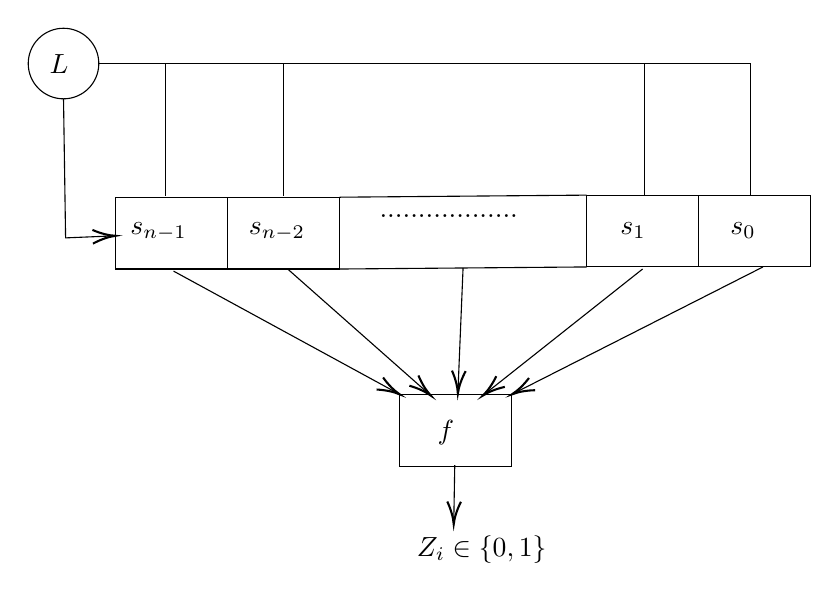
\begin{tikzpicture}[x=0.75pt,y=0.75pt,yscale=-1,xscale=1]
        \draw   (138,1067.4) -- (192,1067.4) -- (192,1102) -- (138,1102) -- cycle ;
        \draw   (192,1067.4) -- (246,1067.4) -- (246,1102) -- (192,1102) -- cycle ;
        \draw   (365,1066.4) -- (419,1066.4) -- (419,1101) -- (365,1101) -- cycle ;
        \draw    (246,1067.4) -- (365,1066.4) ;
        \draw   (419,1066.4) -- (473,1066.4) -- (473,1101) -- (419,1101) -- cycle ; 
        \draw    (246,1102) -- (365,1101) ;
        \draw    (166,1103) -- (273.24,1161.44) ;
        \draw [shift={(275,1162.4)}, rotate = 208.59] [color={rgb, 255:red, 0; green, 0; blue, 0 }  ][line width=0.75]    (10.93,-3.29) .. controls (6.95,-1.4) and (3.31,-0.3) .. (0,0) .. controls (3.31,0.3) and (6.95,1.4) .. (10.93,3.29)   ; 
        \draw    (130,1003) -- (444,1003) -- (444,1066.4) ;
        \draw   (96,1003) .. controls (96,993.61) and (103.61,986) .. (113,986) .. controls (122.39,986) and (130,993.61) .. (130,1003) .. controls (130,1012.39) and (122.39,1020) .. (113,1020) .. controls (103.61,1020) and (96,1012.39) .. (96,1003) -- cycle ;
        \draw    (113,1020) -- (114,1087) -- (136,1086.08) ;
        \draw [shift={(138,1086)}, rotate = 177.61] [color={rgb, 255:red, 0; green, 0; blue, 0 }  ][line width=0.75]    (10.93,-3.29) .. controls (6.95,-1.4) and (3.31,-0.3) .. (0,0) .. controls (3.31,0.3) and (6.95,1.4) .. (10.93,3.29)   ;
        \draw    (162,1003) -- (162,1067) ;
        \draw    (219,1003) -- (219,1067) ; 
        \draw    (393,1003) -- (393,1067) ; 
        \draw   (275,1162.4) -- (329,1162.4) -- (329,1197) -- (275,1197) -- cycle ; 
        \draw    (221,1102) -- (288.5,1161.68) ;
        \draw [shift={(290,1163)}, rotate = 221.48] [color={rgb, 255:red, 0; green, 0; blue, 0 }  ][line width=0.75]    (10.93,-3.29) .. controls (6.95,-1.4) and (3.31,-0.3) .. (0,0) .. controls (3.31,0.3) and (6.95,1.4) .. (10.93,3.29)   ;
        \draw    (392,1102) -- (316.57,1161.76) ;
        \draw [shift={(315,1163)}, rotate = 321.61] [color={rgb, 255:red, 0; green, 0; blue, 0 }  ][line width=0.75]    (10.93,-3.29) .. controls (6.95,-1.4) and (3.31,-0.3) .. (0,0) .. controls (3.31,0.3) and (6.95,1.4) .. (10.93,3.29)   ;
        \draw    (450,1101) -- (330.78,1161.49) ;
        \draw [shift={(329,1162.4)}, rotate = 333.1] [color={rgb, 255:red, 0; green, 0; blue, 0 }  ][line width=0.75]    (10.93,-3.29) .. controls (6.95,-1.4) and (3.31,-0.3) .. (0,0) .. controls (3.31,0.3) and (6.95,1.4) .. (10.93,3.29)   ;
        \draw    (305.5,1101.5) -- (303.08,1160) ;
        \draw [shift={(303,1162)}, rotate = 272.37] [color={rgb, 255:red, 0; green, 0; blue, 0 }  ][line width=0.75]    (10.93,-3.29) .. controls (6.95,-1.4) and (3.31,-0.3) .. (0,0) .. controls (3.31,0.3) and (6.95,1.4) .. (10.93,3.29)   ;
        \draw    (301.5,1196.5) -- (301.04,1223) ;
        \draw [shift={(301,1225)}, rotate = 271.01] [color={rgb, 255:red, 0; green, 0; blue, 0 }  ][line width=0.75]    (10.93,-3.29) .. controls (6.95,-1.4) and (3.31,-0.3) .. (0,0) .. controls (3.31,0.3) and (6.95,1.4) .. (10.93,3.29)   ;
        
        \draw (144,1078.4) node [anchor=north west][inner sep=0.75pt]   [align=left] {$s_{n-1}$};
        \draw (201,1078.4) node [anchor=north west][inner sep=0.75pt]   [align=left] {$s_{n-2}$};
        \draw (264,1074.4) node [anchor=north west][inner sep=0.75pt]   [align=left] {..................};
        \draw (380,1078.4) node [anchor=north west][inner sep=0.75pt]   [align=left] {$s_1$};
        \draw (433,1078.4) node [anchor=north west][inner sep=0.75pt]   [align=left] {$s_0$};
        \draw (105,997.4) node [anchor=north west][inner sep=0.75pt]   [align=left] {$L$};
        \draw (282,1229.4) node [anchor=north west][inner sep=0.75pt]   [align=left] {$Z_i \in \{0,1\}$};
        \draw (292,1173.4) node [anchor=north west][inner sep=0.75pt]   [align=left] {$f$};
    \end{tikzpicture}\\
    \vspace{2mm}
    $f: \{0, 1\}^l \rightarrow \{0, 1\}$\\
    \vspace{1mm}
    $n \geq l$\\
    \vspace{1mm}
    $C_i = m_i \oplus Z_i$
\end{center}

\subsubsection{State Update Function:}
The state update function of the LFSR remains unchanged. It still involves a linear feedback function ($L$) and shifting, as previously described.\\\\
The advantage here is that even if we have $m_i$ and the corresponding $C_i$ from the Known Plaintext Attack model, and thereby know $Z_i$, $Z_i$ becomes a non-linear function of the LFSR's state bits. Solving a non-linear system of equations can present substantial computational hurdles.\\\\
The state update function of LFSR is, say $\alpha$. Therefore, 
\begin{center}
    $S_{t+1} = \alpha(S_t)$\\
    $Z_{t+1} = f(S_{t+1})$
\end{center}
Let us look at the LFSR state at clocking time t.
\begin{center}
    $S_t = (s_{n-1}^t, s_{n-2}^t,....., s_0^t)$
\end{center}
The state of LFSR at clocking time (t+1) will be, 
\begin{center}
    $S_{t+1} = (s_{n-1}^{t+1}, s_{n-2}^{t+1},....., s_0^{t+1})$
\end{center}
Suppose the shifting to be right shift, therefore, 
\begin{center}
    $s_0^{t+1} = s_1^t, s_1^{t+1} = s_2^t,....,s_{n-2}^{t+1} = s_{n-1}^t, s_{n-1}^{t+1} = L(s_{n-1}^t, s_{n-2}^t,....., s_0^t)$
\end{center}
The state update can be represented as a matrix multiplication in the following way,
\begin{center}
    $ S^{t+1} = 
    \begin{bmatrix}
        s_0^{t+1}\\
        s_1^{t+1}\\
        \vdots\\
        S_{n-1}^{t+1}\\
    \end{bmatrix}
    =
    \begin{bmatrix}
        0 & 1 & 0 & 0 & \hdots & 0\\
        0 & 0 & 1 & 0 & \hdots & 0\\
        0 & 0 & 0 & 1 & \hdots & 0\\
        \vdots & \vdots & \vdots & \vdots & \ddots & \vdots\\
        0 & 0 & 0 & 0 & \hdots & 1\\
        c_n & c_{n-1} & c_{n-2} & c_{n-3} & \hdots & c_1\\
    \end{bmatrix}
    \begin{bmatrix}
        s_0^{t}\\
        s_1^{t}\\
        \vdots\\
        S_{n-1}^{t}\\
    \end{bmatrix}
    $\\
    \vspace{2mm}
    $L = c_n\cdot s_0 \oplus c_{n-1} \cdot s_1 \oplus \hdots \oplus c_1\cdot s_{n-1}$
\end{center}


\subsection{LFSR With Combiner Function}

We utilize a function $f$ resembling the one described earlier. However, in this scenario, we incorporate $l$ Linear Feedback Shift Registers (LFSRs). The outputs of these $l$ LFSRs, forming $l$ bits, are inputted into the combiner function $f$, resulting in an output denoted as $Z_i$. It's important to emphasize that function $f$ remains nonlinear in this context.

\begin{center}
    \tikzset{every picture/.style={line width=0.75pt}}
    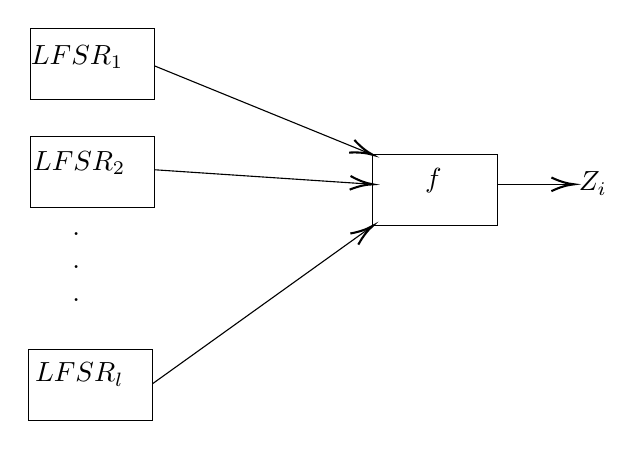
\begin{tikzpicture}[x=0.75pt,y=0.75pt,yscale=-1,xscale=1]
        \draw   (121,47) -- (181,47) -- (181,81.2) -- (121,81.2) -- cycle ;
        \draw   (120,202) -- (180,202) -- (180,236.2) -- (120,236.2) -- cycle ;
        \draw   (121,99) -- (181,99) -- (181,133.2) -- (121,133.2) -- cycle ;
        \draw   (286,108) -- (346,108) -- (346,142.2) -- (286,142.2) -- cycle ;
        \draw    (181,65.2) -- (284.15,107.25) ;
        \draw [shift={(286,108)}, rotate = 202.18] [color={rgb, 255:red, 0; green, 0; blue, 0 }  ][line width=0.75]    (10.93,-3.29) .. controls (6.95,-1.4) and (3.31,-0.3) .. (0,0) .. controls (3.31,0.3) and (6.95,1.4) .. (10.93,3.29)   ;
        \draw    (181,115.2) -- (284,122.07) ;
        \draw [shift={(286,122.2)}, rotate = 183.81] [color={rgb, 255:red, 0; green, 0; blue, 0 }  ][line width=0.75]    (10.93,-3.29) .. controls (6.95,-1.4) and (3.31,-0.3) .. (0,0) .. controls (3.31,0.3) and (6.95,1.4) .. (10.93,3.29)   ;
        \draw    (180,218.2) -- (284.37,143.37) ;
        \draw [shift={(286,142.2)}, rotate = 144.36] [color={rgb, 255:red, 0; green, 0; blue, 0 }  ][line width=0.75]    (10.93,-3.29) .. controls (6.95,-1.4) and (3.31,-0.3) .. (0,0) .. controls (3.31,0.3) and (6.95,1.4) .. (10.93,3.29)   ;
        \draw    (346,122.2) -- (381,122.2) ;
        \draw [shift={(383,122.2)}, rotate = 180] [color={rgb, 255:red, 0; green, 0; blue, 0 }  ][line width=0.75]    (10.93,-3.29) .. controls (6.95,-1.4) and (3.31,-0.3) .. (0,0) .. controls (3.31,0.3) and (6.95,1.4) .. (10.93,3.29)   ;
        
        \draw (120,54) node [anchor=north west][inner sep=0.75pt]   [align=left] {$LFSR_1$};
        \draw (121,105) node [anchor=north west][inner sep=0.75pt]   [align=left] {$LFSR_2$};
        \draw (122,207) node [anchor=north west][inner sep=0.75pt]   [align=left] {$LFSR_l$};
        \draw (310,113) node [anchor=north west][inner sep=0.75pt]   [align=left] {$f$};
        \draw (140,144) node [anchor=north west][inner sep=0.75pt]   [align=left] {.\\.\\.};
        \draw (384,115) node [anchor=north west][inner sep=0.75pt]   [align=left] {$Z_i$};
    \end{tikzpicture}\\
    $C_i = m_i \oplus Z_i$
\end{center}
\subsection*{Example:}

Consider the following 3-LFSR with nonlinear filter function $f$.
\begin{center}
    \tikzset{every picture/.style={line width=0.75pt}}       
    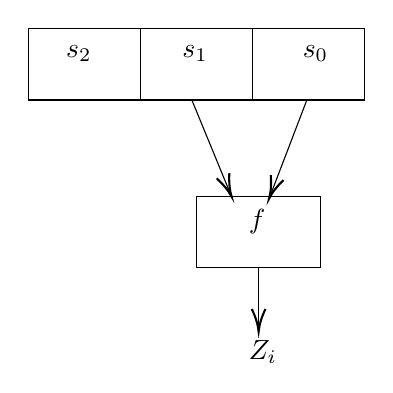
\begin{tikzpicture}[x=0.75pt,y=0.75pt,yscale=-1,xscale=1]
        \draw   (444,57) -- (498,57) -- (498,91.6) -- (444,91.6) -- cycle ;
        \draw   (498,57) -- (552,57) -- (552,91.6) -- (498,91.6) -- cycle ;
        \draw   (552,57) -- (606,57) -- (606,91.6) -- (552,91.6) -- cycle ;
        \draw   (525,138) -- (585,138) -- (585,172.2) -- (525,172.2) -- cycle ;
        \draw    (523,92) -- (541.24,136.35) ;
        \draw [shift={(542,138.2)}, rotate = 247.64] [color={rgb, 255:red, 0; green, 0; blue, 0 }  ][line width=0.75]    (10.93,-3.29) .. controls (6.95,-1.4) and (3.31,-0.3) .. (0,0) .. controls (3.31,0.3) and (6.95,1.4) .. (10.93,3.29)   ;
        \draw    (578,92.2) -- (560.72,137.33) ;
        \draw [shift={(560,139.2)}, rotate = 290.96] [color={rgb, 255:red, 0; green, 0; blue, 0 }  ][line width=0.75]    (10.93,-3.29) .. controls (6.95,-1.4) and (3.31,-0.3) .. (0,0) .. controls (3.31,0.3) and (6.95,1.4) .. (10.93,3.29)   ;
        \draw    (555,172) -- (555,201.2) ;
        \draw [shift={(555,203.2)}, rotate = 270] [color={rgb, 255:red, 0; green, 0; blue, 0 }  ][line width=0.75]    (10.93,-3.29) .. controls (6.95,-1.4) and (3.31,-0.3) .. (0,0) .. controls (3.31,0.3) and (6.95,1.4) .. (10.93,3.29)   ;
        
        \draw (517,64) node [anchor=north west][inner sep=0.75pt]   [align=left] {$s_1$};
        \draw (461,64) node [anchor=north west][inner sep=0.75pt]   [align=left] {$s_2$};
        \draw (575,64) node [anchor=north west][inner sep=0.75pt]   [align=left] {$s_0$};
        \draw (549,143) node [anchor=north west][inner sep=0.75pt]   [align=left] {$f$};
        \draw (549,206) node [anchor=north west][inner sep=0.75pt]   [align=left] {$Z_i$};
    \end{tikzpicture}\\
    $f: \{0,1\}^2 \rightarrow \{0,1\}$\\
    $f(x_0, x_1) = x_0 \cdot x_1$
\end{center}

\noindent
\textbf{Solution:}\\\\
Here, if we draw the truth table of $f$, it will look like,
\[
\begin{array}{ccc}
x_0 & x_1 & f \\
0 & 0 & 0 \\
0 & 1 & 0 \\
1 & 0 & 0 \\
1 & 1 & 1 \\
\end{array}
\]\\
Noting that $Pr[Z = 0] = \frac{3}{4}$, we conclude that $f$ does not exhibit ideal behavior since $Pr[Z = 0]$ exceeds $Pr[Z = 1]$, indicating a notable bias. It's crucial to devise $f$ in a manner that guarantees unpredictability in the output. Currently, predicting an output of zero is more likely. If such a model were employed in a stream cipher and we managed to ascertain the function $f$, it would expose the stream cipher to vulnerabilities. Therefore, the selection of $f$ must be approached cautiously to mitigate such risks.

\subsection{Non-Linear Feedback Shift Register (NFSR)}

In NFSR, the mechanism is similar to LFSR, but the feedback is non-linear.

\[ f : \{0, 1\}^l \rightarrow \{0, 1\} \]

\section{Hash Function}

A hash function is a mapping from one set to another set with certain properties.

\[ h : A \rightarrow B \]
\[ h(X) = Y \]

\subsection{Properties of Hash Function}
\begin{enumerate}
    \item If \( X \) is altered to \( X' \), then \( h(X') \) will be completely different from \( h(X) \).
    \item Given \( Y \), it is practically infeasible to find \( X \) such that \( h(X) = Y \).
    \item Given \( X \) and \( Y = h(X) \), it is practically infeasible to find \( X' \) such that \( h(X) = h(X') \).
\end{enumerate}
\noindent
Consider a scenario
\begin{center}
    

\tikzset{every picture/.style={line width=0.75pt}} %set default line width to 0.75pt        

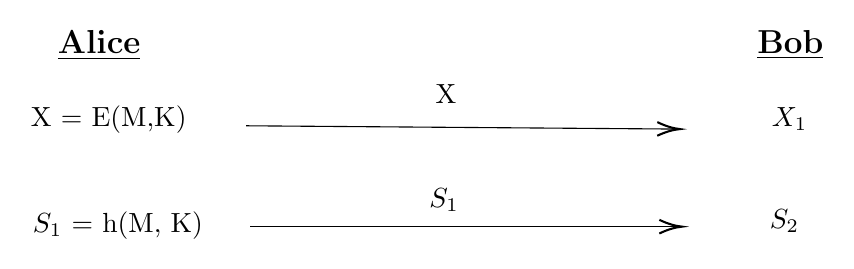
\begin{tikzpicture}[x=0.75pt,y=0.75pt,yscale=-1,xscale=1]
%uncomment if require: \path (0,300); %set diagram left start at 0, and has height of 300

%Straight Lines [id:da6936070700935975] 
\draw    (247,132) -- (454,133.58) ;
\draw [shift={(456,133.6)}, rotate = 180.44] [color={rgb, 255:red, 0; green, 0; blue, 0 }  ][line width=0.75]    (10.93,-3.29) .. controls (6.95,-1.4) and (3.31,-0.3) .. (0,0) .. controls (3.31,0.3) and (6.95,1.4) .. (10.93,3.29)   ;
%Straight Lines [id:da1977592175436449] 
\draw    (249,180.6) -- (455,180.6) ;
\draw [shift={(457,180.6)}, rotate = 180] [color={rgb, 255:red, 0; green, 0; blue, 0 }  ][line width=0.75]    (10.93,-3.29) .. controls (6.95,-1.4) and (3.31,-0.3) .. (0,0) .. controls (3.31,0.3) and (6.95,1.4) .. (10.93,3.29)   ;

% Text Node
\draw (155,85) node [anchor=north west][inner sep=0.75pt]   [align=left] {\textbf{{\large \underline{Alice}}}};
% Text Node
\draw (492,85) node [anchor=north west][inner sep=0.75pt]   [align=left] {\textbf{\underline{{\large Bob}}}};
% Text Node
\draw (142,121) node [anchor=north west][inner sep=0.75pt]   [align=left] {X = E(M,K)};
% Text Node
\draw (499,122) node [anchor=north west][inner sep=0.75pt]   [align=left] {$X_1$};
% Text Node
\draw (143,172) node [anchor=north west][inner sep=0.75pt]   [align=left] {$S_1$ = h(M, K)};
% Text Node
\draw (498,171) node [anchor=north west][inner sep=0.75pt]   [align=left] {$S_2$};
% Text Node
\draw (337,111) node [anchor=north west][inner sep=0.75pt]   [align=left] {X};
% Text Node
\draw (334,161) node [anchor=north west][inner sep=0.75pt]   [align=left] {$S_1$};


\end{tikzpicture}

\end{center}
\noindent
If \( h(X_1,K) = S_2 \), then Bob will accept \( X_1 \).
We are able to check whether X Is altered during communication.

\subsection{Formal definition of Hash Function}
A hash family is a four-tuple \( (P, S, K, H) \) where the following conditions are satisfied:
\begin{enumerate}
    \item \( P \) is the set of all possible messages.
    \item \( S \) is the set of all possible message digests or authentication tags (all output).
    \item \( K \) is the key space.
    \item For each \( K_i \in K \), there is a hash function \( h_{K_i} \) such that \( h_{K_i} : P \rightarrow S \), where \( |P| \geq |S| \) and more interestingly \( |P| \geq 2 \times |S| \).
\end{enumerate}

\subsection{Types of Hash Function}
\begin{center}
    

\begin{forest}
for tree={
    parent anchor=south,
    child anchor=north,
    align=center,
    edge={->},
    l sep+=20pt,
}
[\textbf{TYPES OF HASH FUNCTION}
    [\textbf{Keyed Hash function}
        [If a key is involved\\in the computation\\of the hash value]
    ]
    [\textbf{Unkeyed Hash function}
        [If a key is not involved\\in the computation\\of the hash value]
    ]
]
\end{forest}
\end{center}

\subsection{Essential Problems}
\begin{enumerate}
    \item \textbf{Pre-Image Finding Problem:} Given a hash function \( h : P \rightarrow S \) and \( y \in S \), find \( x \in P \) such that \( h(x) = y \).
    \item \textbf{Second Pre-Image Finding Problem:} Given a hash function \( h : P \rightarrow S \), \( x \in P \), and \( h(x) \), find \( x' \in P \) such that \( x' \neq x \) and \( h(x') = h(x) \).
    \item \textbf{Collision Finding Problem:} Given a hash function \( h \), find \( x, x' \in P \) such that \( x \neq x' \) and \( h(x) = h(x') \).
\end{enumerate}

\fbox{\parbox{\linewidth}{
{\textbf{Ideal Hash Function:}\\\\}
An ideal hash function \( h : P \rightarrow S \) will be called ideal if given \( x \in P \), to find \( h(x) \), either we have to apply \( h \) on \( x \) or we have to look into the table corresponding to \( h \) (hash table).
}}


\subsection{Algorithms for the formulated problems}
\subsubsection{Pre-Image Finding Algorithm}
\textbf{Given:} \( y \in Y \) \\\\
\textbf{Find:} \( x \in X \) such that \( h(x) = y \)\\\\
\begin{algorithm}[H]
\SetAlgoLined
\KwResult{Pre-image \( x \)}
\( h : X \rightarrow Y \) \\
Choose any \( X_0 \subseteq X \) such that \( |X_0| = Q \) for each \( x \in X_0 \) \\
Compute \( y_x = h(x) \) \\
\eIf{\( y_x = y \)}{
Return \( x \)}{
Continue}
\end{algorithm}
\noindent
\\Pr [the above algorithm returns correct pre-image] - gives you the complexity.\\\\
Let us find the probability of finding pre-image using $X_o$\\
\begin{center}
    $X_o = \{x_1, x_2, \dots , x_Q \}$\\
    $E_i : event h(x_i) = y; 1 \leq i \leq Q$
\end{center}
\noindent
\\h(x) can have M values, out of which only one will give success. So,
\begin{center}
    $Pr[E_i] = \frac{1}{M}$\\
    $Pr[{E_i}'] = 1- \frac{1}{M}$
\end{center}
\noindent
\\Now we accumulate the probabilities of $E_1, E_2 \dots E_Q$
\begin{center}
    $Pr[E_1 \cup E_2 \cup E_3 \cup \dots \cup E_Q] = 1 - Pr[{E_1}' \cap {E_2}' \cap {E_3}' \cap \dots \cap {E_Q}']$\\
    \vspace{3mm}
    $Pr[E_1 \cup E_2 \cup E_3 \cup \dots \cup E_Q] = 1 - \prod_{i=1}^{Q} Pr[{E_i}']$\\
    \vspace{3mm}
    $Pr[E_1 \cup E_2 \cup E_3 \cup \dots \cup E_Q] = 1 - {(1-\frac{1}{M})}^Q$
\end{center}
Let us expand it now. 
\begin{center}
    $Pr[E_1 \cup E_2 \cup E_3 \cup \dots \cup E_Q] = 1 - [1-(\binom{Q}{1} \frac{1}{M} + \binom{Q}{2} \frac{1}{M^2} \dots]$\\
    \vspace{3mm}
    $Pr[E_1 \cup E_2 \cup E_3 \cup \dots \cup E_Q] \approx  1 - [1-(\binom{Q}{1} \frac{1}{M}]$\\
    \vspace{3mm}
    $Pr[E_1 \cup E_2 \cup E_3 \cup \dots \cup E_Q] \approx \frac{Q}{M}$
\end{center}
Therefore, 
\begin{center}
    Pr[ pre image finding ] = $\frac{Q}{M}$\\
    \vspace{3mm}
    Complexity(pre image finding) = O(M)
\end{center}

%%%%%%%%%%%%%%%%%%%%%%%%%%%%%%%%%%%%%%%%%%%%
%END
 
\end{document}